\documentclass[12pt,a4paper]{article}

\usepackage[a4paper,margin=1in]{geometry}
\usepackage{graphicx}
\usepackage{booktabs}
\usepackage{amsmath,amssymb}
\usepackage{float}
\usepackage{hyperref}
\usepackage{xurl}
\usepackage{xcolor}
\usepackage{listings}
\usepackage{enumitem}
\usepackage{fancyhdr}
\usepackage{longtable}

\hypersetup{colorlinks=true,linkcolor=blue,urlcolor=blue}

\pagestyle{fancy}
\fancyhf{}
\lhead{ICS1512}
\rhead{Machine Learning Algorithms Laboratory}
\cfoot{\thepage}

\setlength{\parskip}{0.4em}
\setlength{\parindent}{0pt}
\setlength{\headheight}{15pt}

\setlength{\floatsep}{10pt plus 2pt minus 2pt}
\setlength{\textfloatsep}{12pt plus 2pt minus 2pt}
\setlength{\intextsep}{10pt plus 2pt minus 2pt}

\setcounter{topnumber}{3}
\setcounter{bottomnumber}{3}
\setcounter{totalnumber}{4}
\renewcommand{\topfraction}{0.85}
\renewcommand{\bottomfraction}{0.85}
\renewcommand{\textfraction}{0.15}
\renewcommand{\floatpagefraction}{0.8}

\lstset{
language=Python,
basicstyle=\ttfamily\small,
numbers=left,
frame=single,
breaklines=true,
showstringspaces=false
}

\begin{document}

\begin{tabular}{|p{4cm}|p{11cm}|}
\hline
Experiment No. & 1 \\ \hline
Experiment Title & Working with Python Packages: NumPy, SciPy, Scikit-Learn, Matplotlib, and Pandas (Predicting Diabetes Dataset) \\ \hline
Student Name & Srinivasan M \\ \hline
Register Number & 3122247001063 \\ \hline
Faculty & Dr. Poreddy Ajay Kumar Reddy \\ \hline
Submission Date & \today \\ \hline
\end{tabular}

\vspace{0.3cm}

\section{Objective}
The key objectives for the Diabetes dataset analysis include:
\begin{itemize}[noitemsep]
    \item Conduct automated exploratory data profiling on clinical attributes from the Pima Indians Diabetes dataset.
    \item Detect physiological data anomalies (e.g. zero values in blood pressure or insulin) and evaluate diagnostic target imbalance.
    \item Generate diagnostic figures into \texttt{figures\_diabetes/}.
\end{itemize}

\section{Problem Statement}
Medical diagnostic datasets often present hidden physiological anomalies (such as recorded zero values for physiological parameters like Glucose, BMI, or Insulin) alongside class imbalance. Manual inspection can miss subtle distributional biases. Implementing an automated EDA utility allows rapid identification of data entry errors, attribute distributions, and diagnostic correlation signals.

\section{Dataset Description}
The **Pima Indians Diabetes Dataset** contains 768 female patient records evaluated for diabetes status.

\begin{longtable}{|p{6cm}|p{8cm}|}
\hline
Dataset Name & Pima Indians Diabetes Dataset \\ \hline
Dataset Source & National Institute of Diabetes and Digestive and Kidney Diseases / Kaggle \\ \hline
Number of Samples & 768 \\ \hline
Number of Features & 8 numerical clinical attributes \\ \hline
Target Attribute & \texttt{Outcome} (0 = Non-diabetic, 1 = Diabetic) \\ \hline
Missing Values & Physiological zeros present in Glucose, BloodPressure, SkinThickness, Insulin, BMI \\ \hline
Train-Test Split & N/A (Exploratory Phase) \\ \hline
\end{longtable}

Features in this dataset:
\begin{itemize}[noitemsep]
    \item \texttt{Pregnancies}: Number of times pregnant.
    \item \texttt{Glucose}: Plasma glucose concentration at 2 hours in an oral glucose tolerance test.
    \item \texttt{BloodPressure}: Diastolic blood pressure (mm Hg).
    \item \texttt{SkinThickness}: Triceps skin fold thickness (mm).
    \item \texttt{Insulin}: 2-Hour serum insulin ($\mu$U/ml).
    \item \texttt{BMI}: Body mass index ($\text{weight in kg}/(\text{height in m})^2$).
    \item \texttt{DiabetesPedigreeFunction}: Diabetes pedigree genetic function score.
    \item \texttt{Age}: Patient age in years.
    \item \texttt{Outcome}: Class variable (0 or 1).
\end{itemize}

\section{Exploratory Data Analysis}
The automated EDA framework produced 29 diagnostic plots saved in \texttt{figures\_diabetes/}.

\subsection{Histograms of Numerical Features}

\begin{figure}[H]
\centering
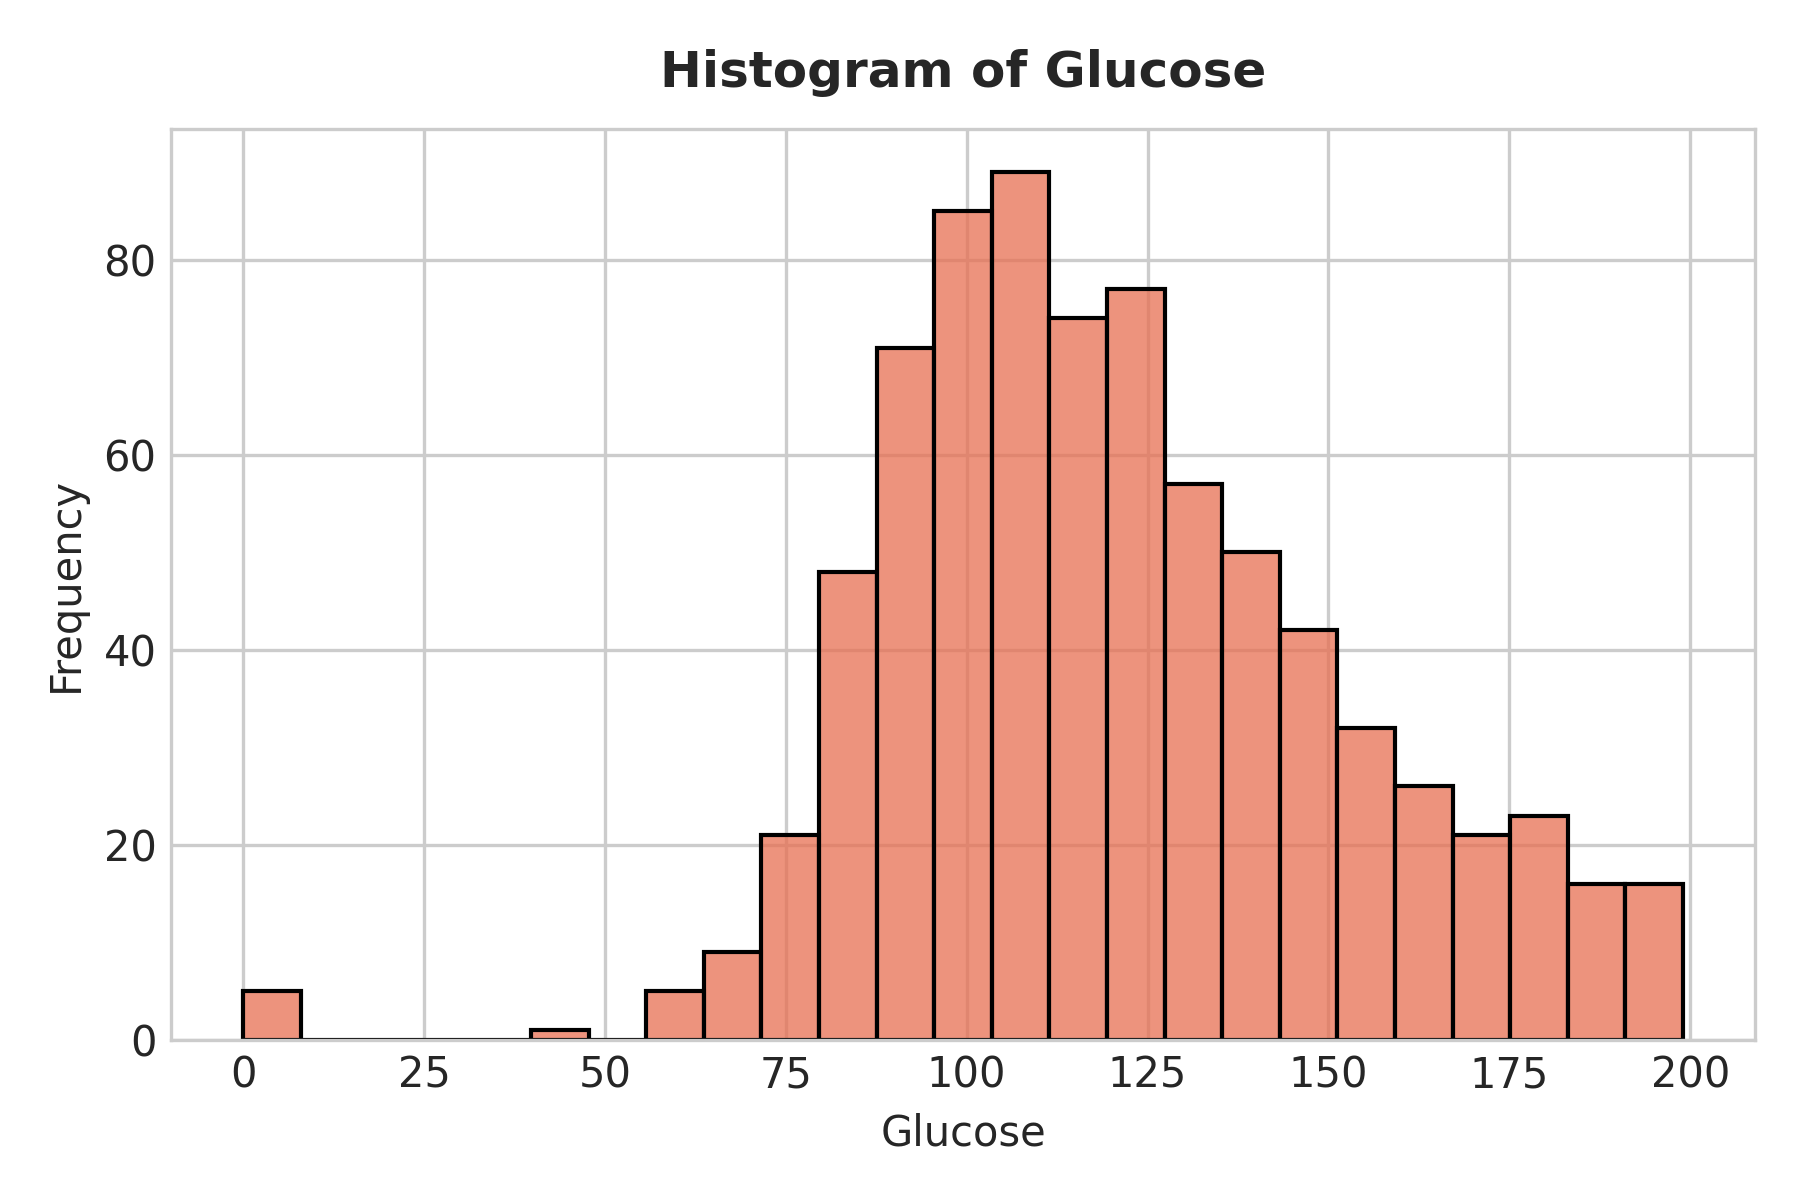
\includegraphics[width=0.75\linewidth]{figures_diabetes/hist_Glucose.png}
\caption{Histogram of Plasma Glucose Levels}
\label{fig:diab_hist_glucose}
\end{figure}
\textbf{Inference:} Glucose levels follow a unimodal normal curve centered near 120 mg/dL. A small spike at 0 mg/dL indicates invalid missing measurements requiring median imputation.

\begin{figure}[H]
\centering
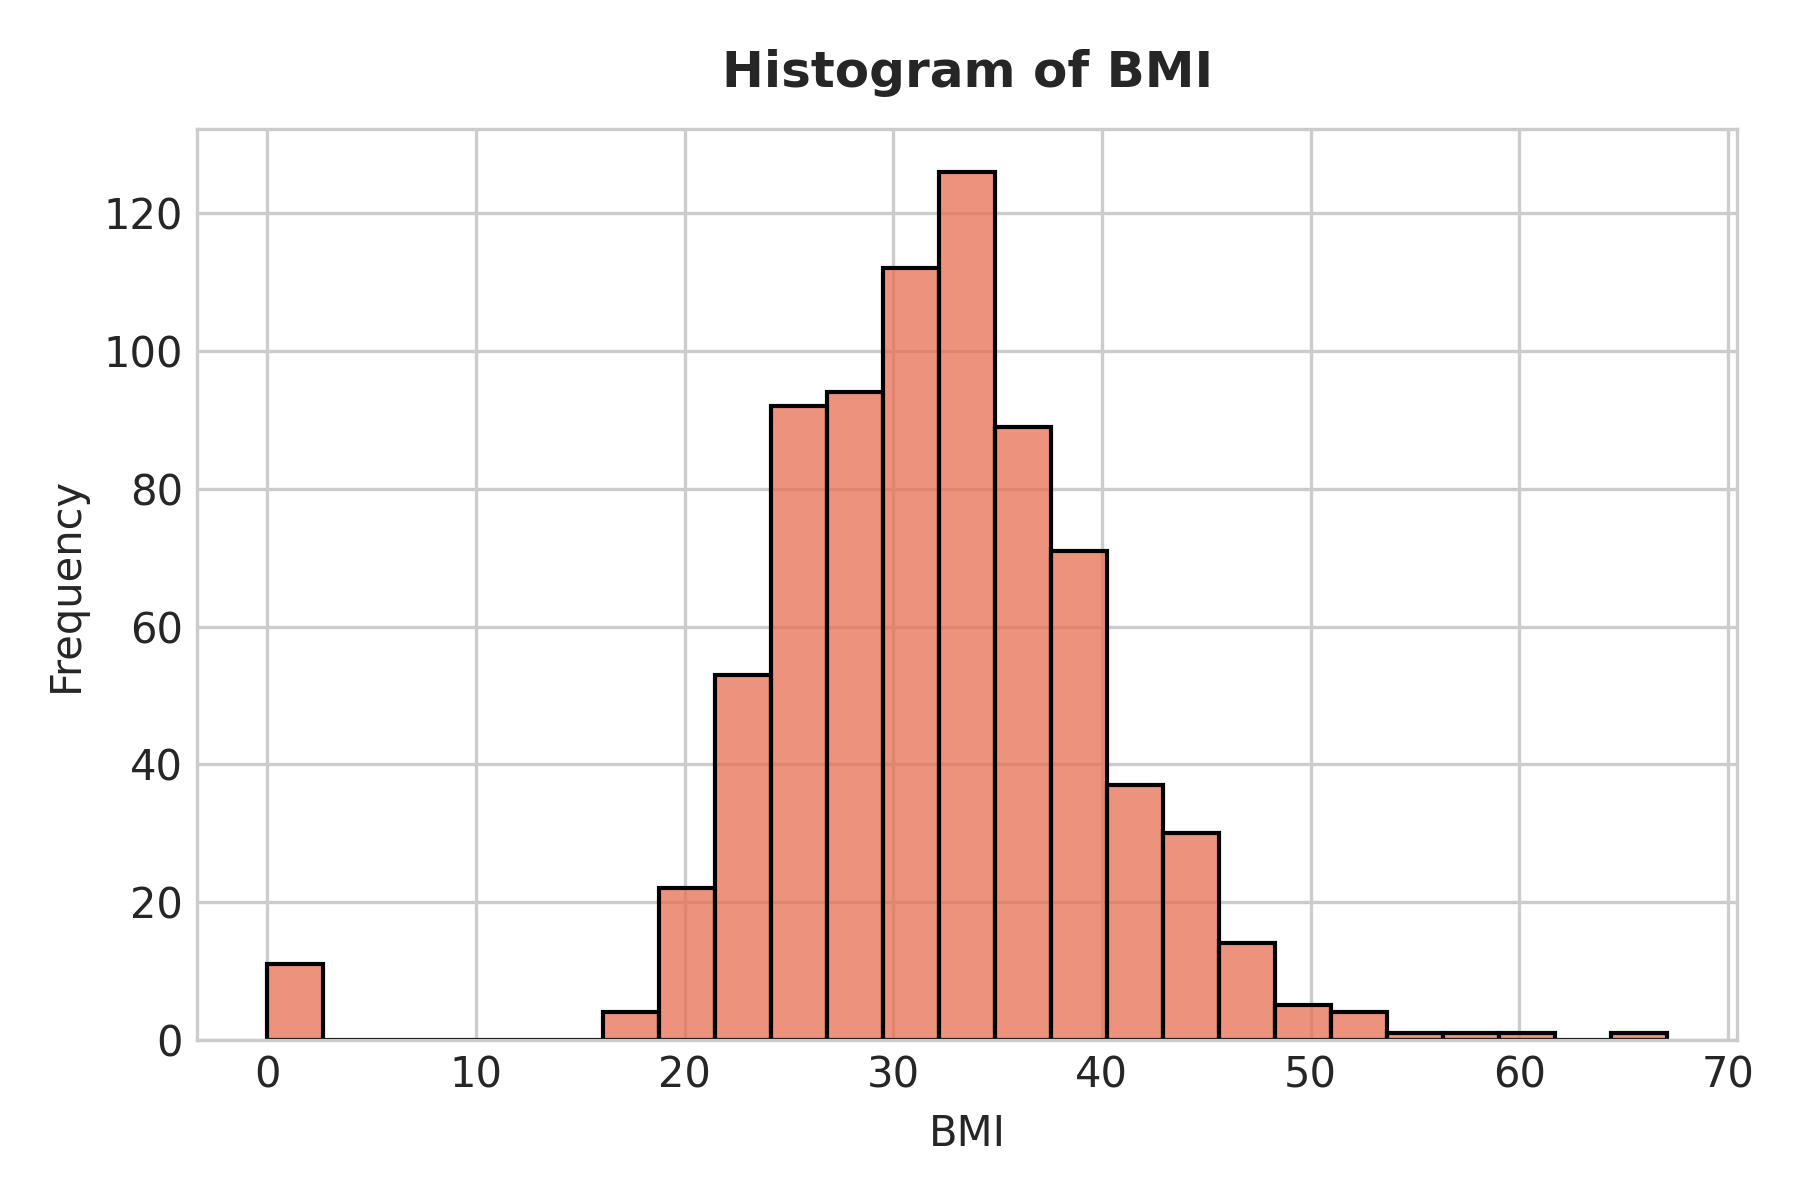
\includegraphics[width=0.75\linewidth]{figures_diabetes/hist_BMI.png}
\caption{Histogram of Body Mass Index (BMI)}
\label{fig:diab_hist_bmi}
\end{figure}
\textbf{Inference:} BMI exhibits a bell-shaped distribution peaking around 32--34 $\text{kg/m}^2$, with several zero values representing missing medical entries.

\subsection{Box Plots by Diagnostic Outcome}

\begin{figure}[H]
\centering
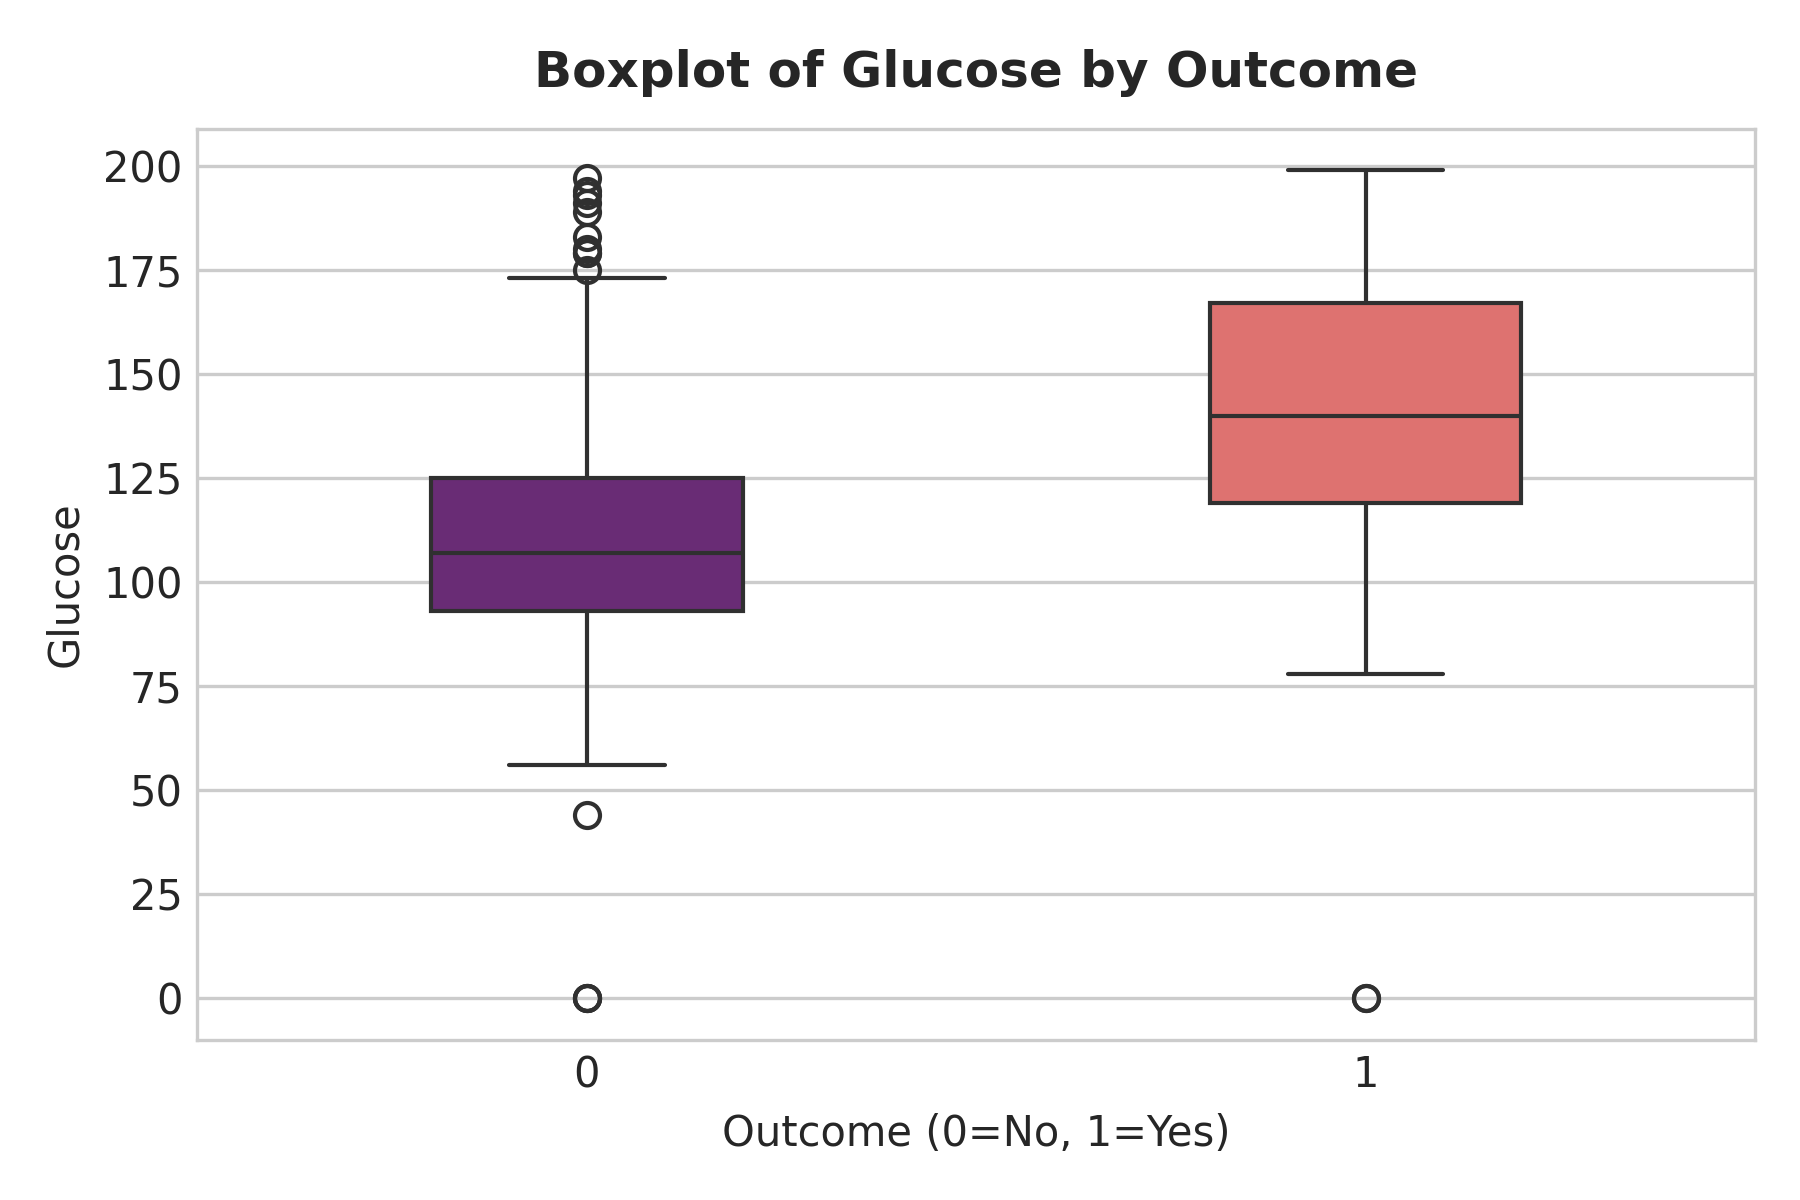
\includegraphics[width=0.75\linewidth]{figures_diabetes/box_Glucose.png}
\caption{Box Plot of Glucose by Diabetes Outcome}
\label{fig:diab_box_glucose}
\end{figure}
\textbf{Inference:} Patients diagnosed with diabetes (\texttt{Outcome} = 1) exhibit significantly higher median glucose levels ($\approx 140$ mg/dL) compared to non-diabetic individuals ($\approx 107$ mg/dL).

\subsection{Kernel Density Estimation (KDE) Plots}

\begin{figure}[H]
\centering
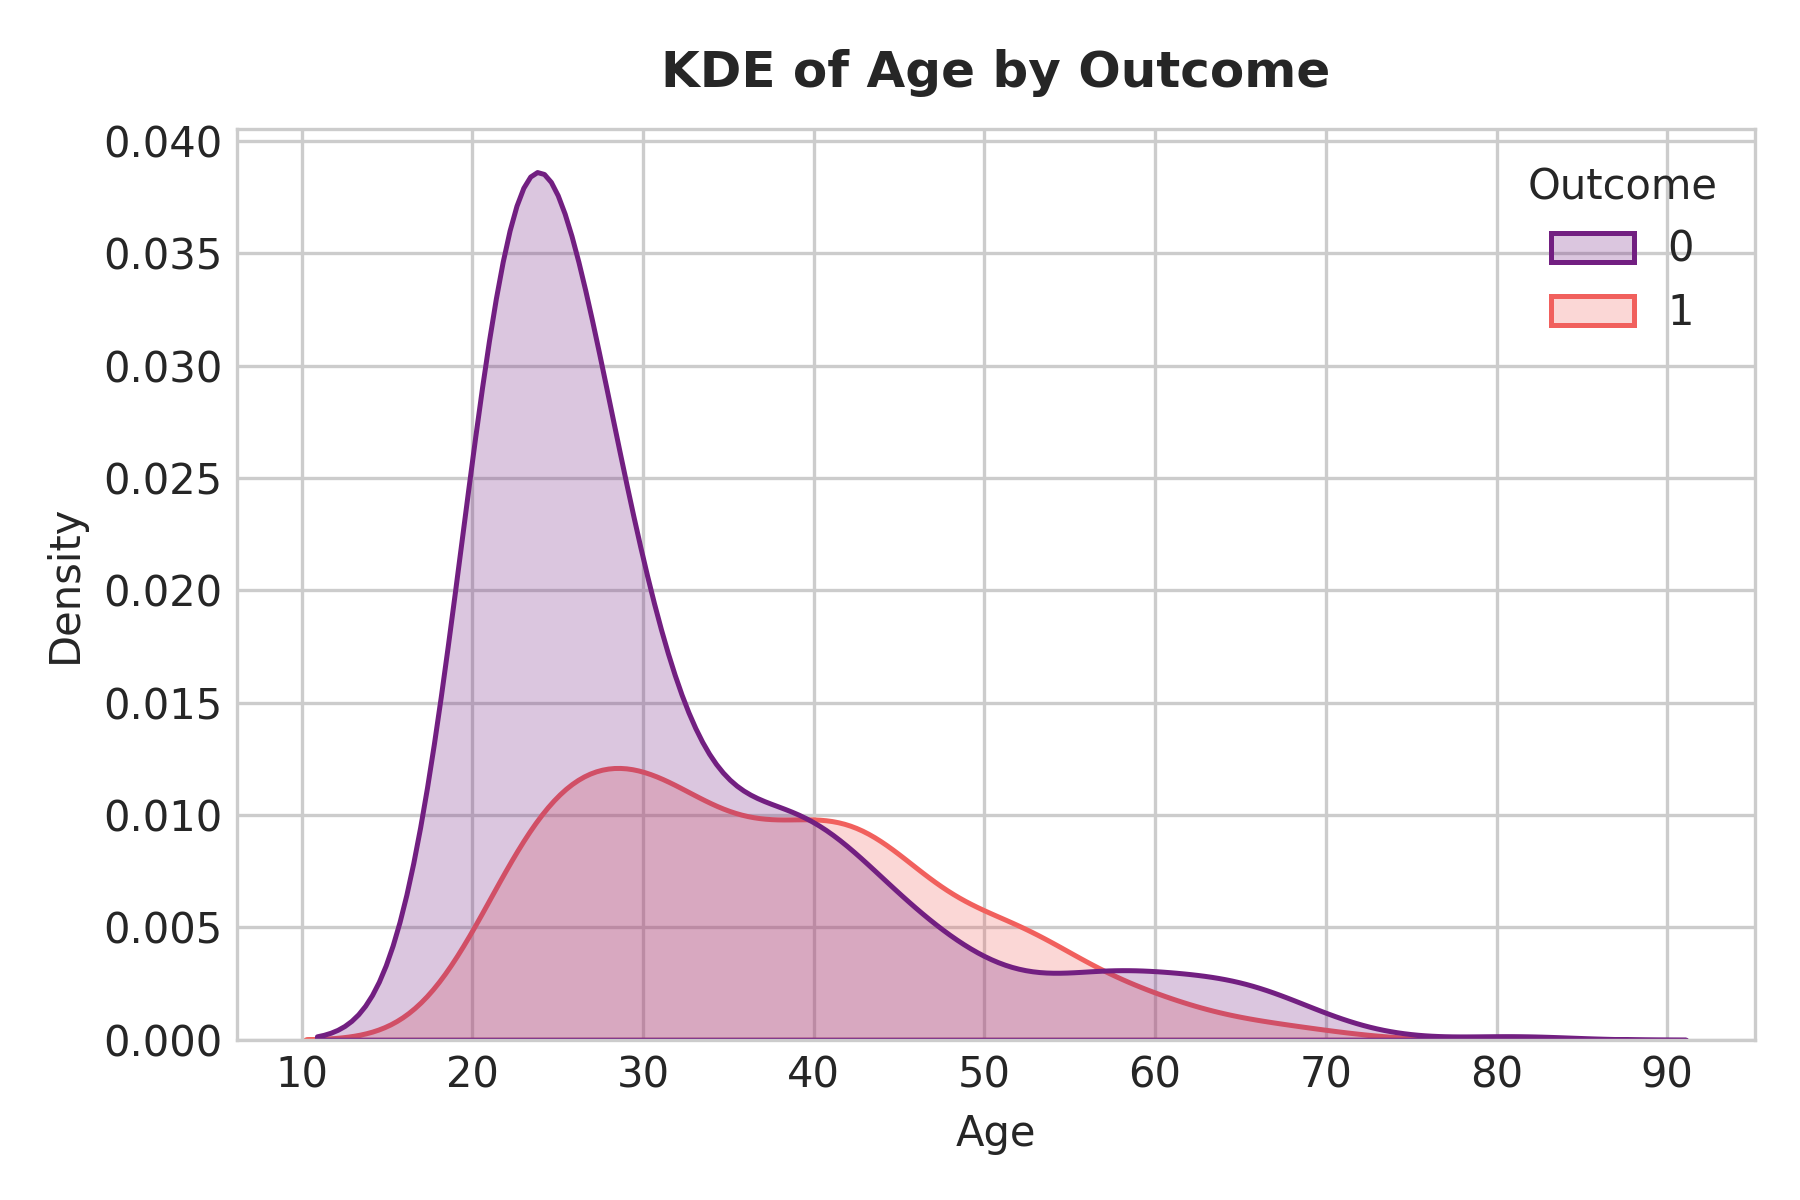
\includegraphics[width=0.75\linewidth]{figures_diabetes/kde_Age.png}
\caption{KDE Density of Age by Outcome}
\label{fig:diab_kde_age}
\end{figure}
\textbf{Inference:} Non-diabetic patients concentrate heavily in the 20--30 age group, whereas diabetic cases show a broader distribution extending into 40--60 years.

\subsection{Count Plots of Categorical Features}

\begin{figure}[H]
\centering
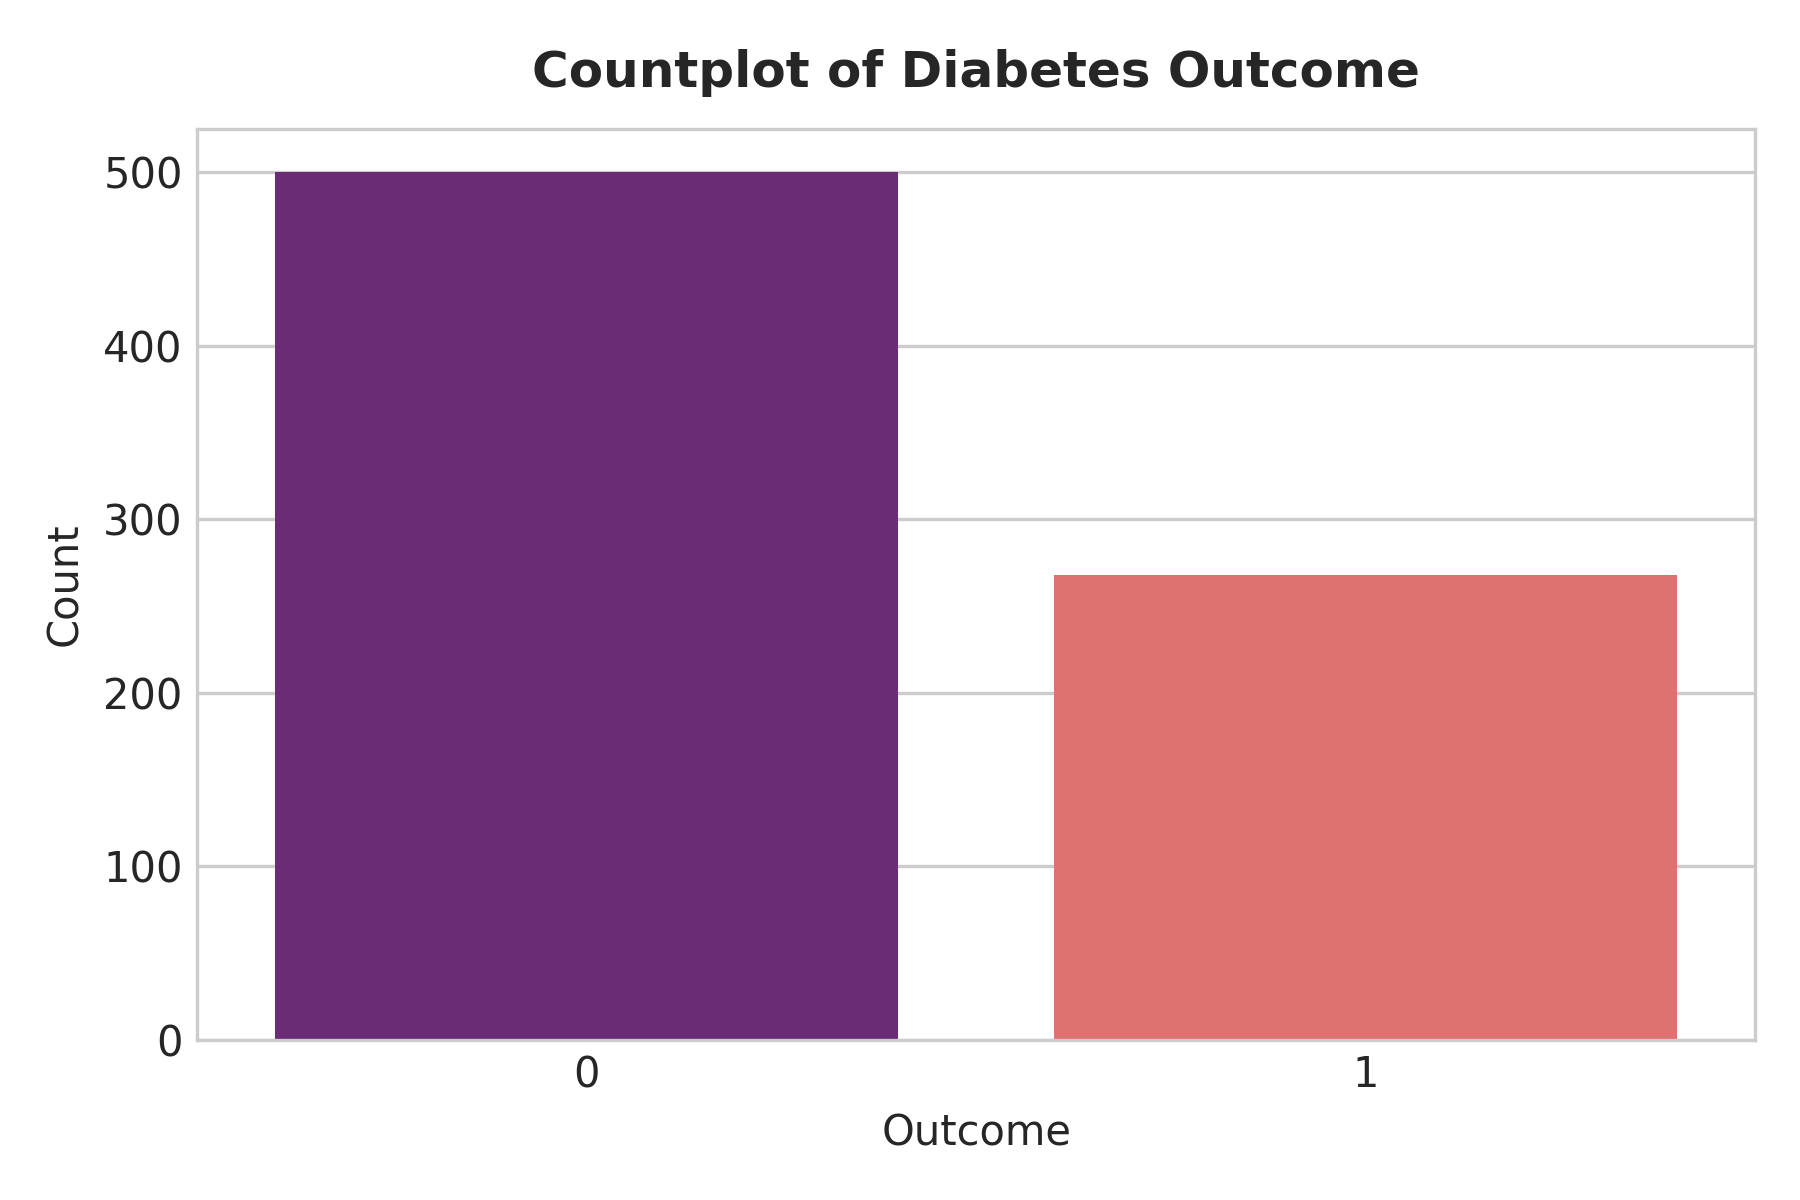
\includegraphics[width=0.75\linewidth]{figures_diabetes/count_Outcome.png}
\caption{Count Plot of Diabetes Outcome}
\label{fig:diab_count_outcome}
\end{figure}
\textbf{Inference:} Out of 768 patients, 500 (65.1\%) are non-diabetic (0) and 268 (34.9\%) are diabetic (1), indicating a moderate class imbalance.

\subsection{Correlation Heatmap of Numerical Features}

\begin{figure}[H]
\centering
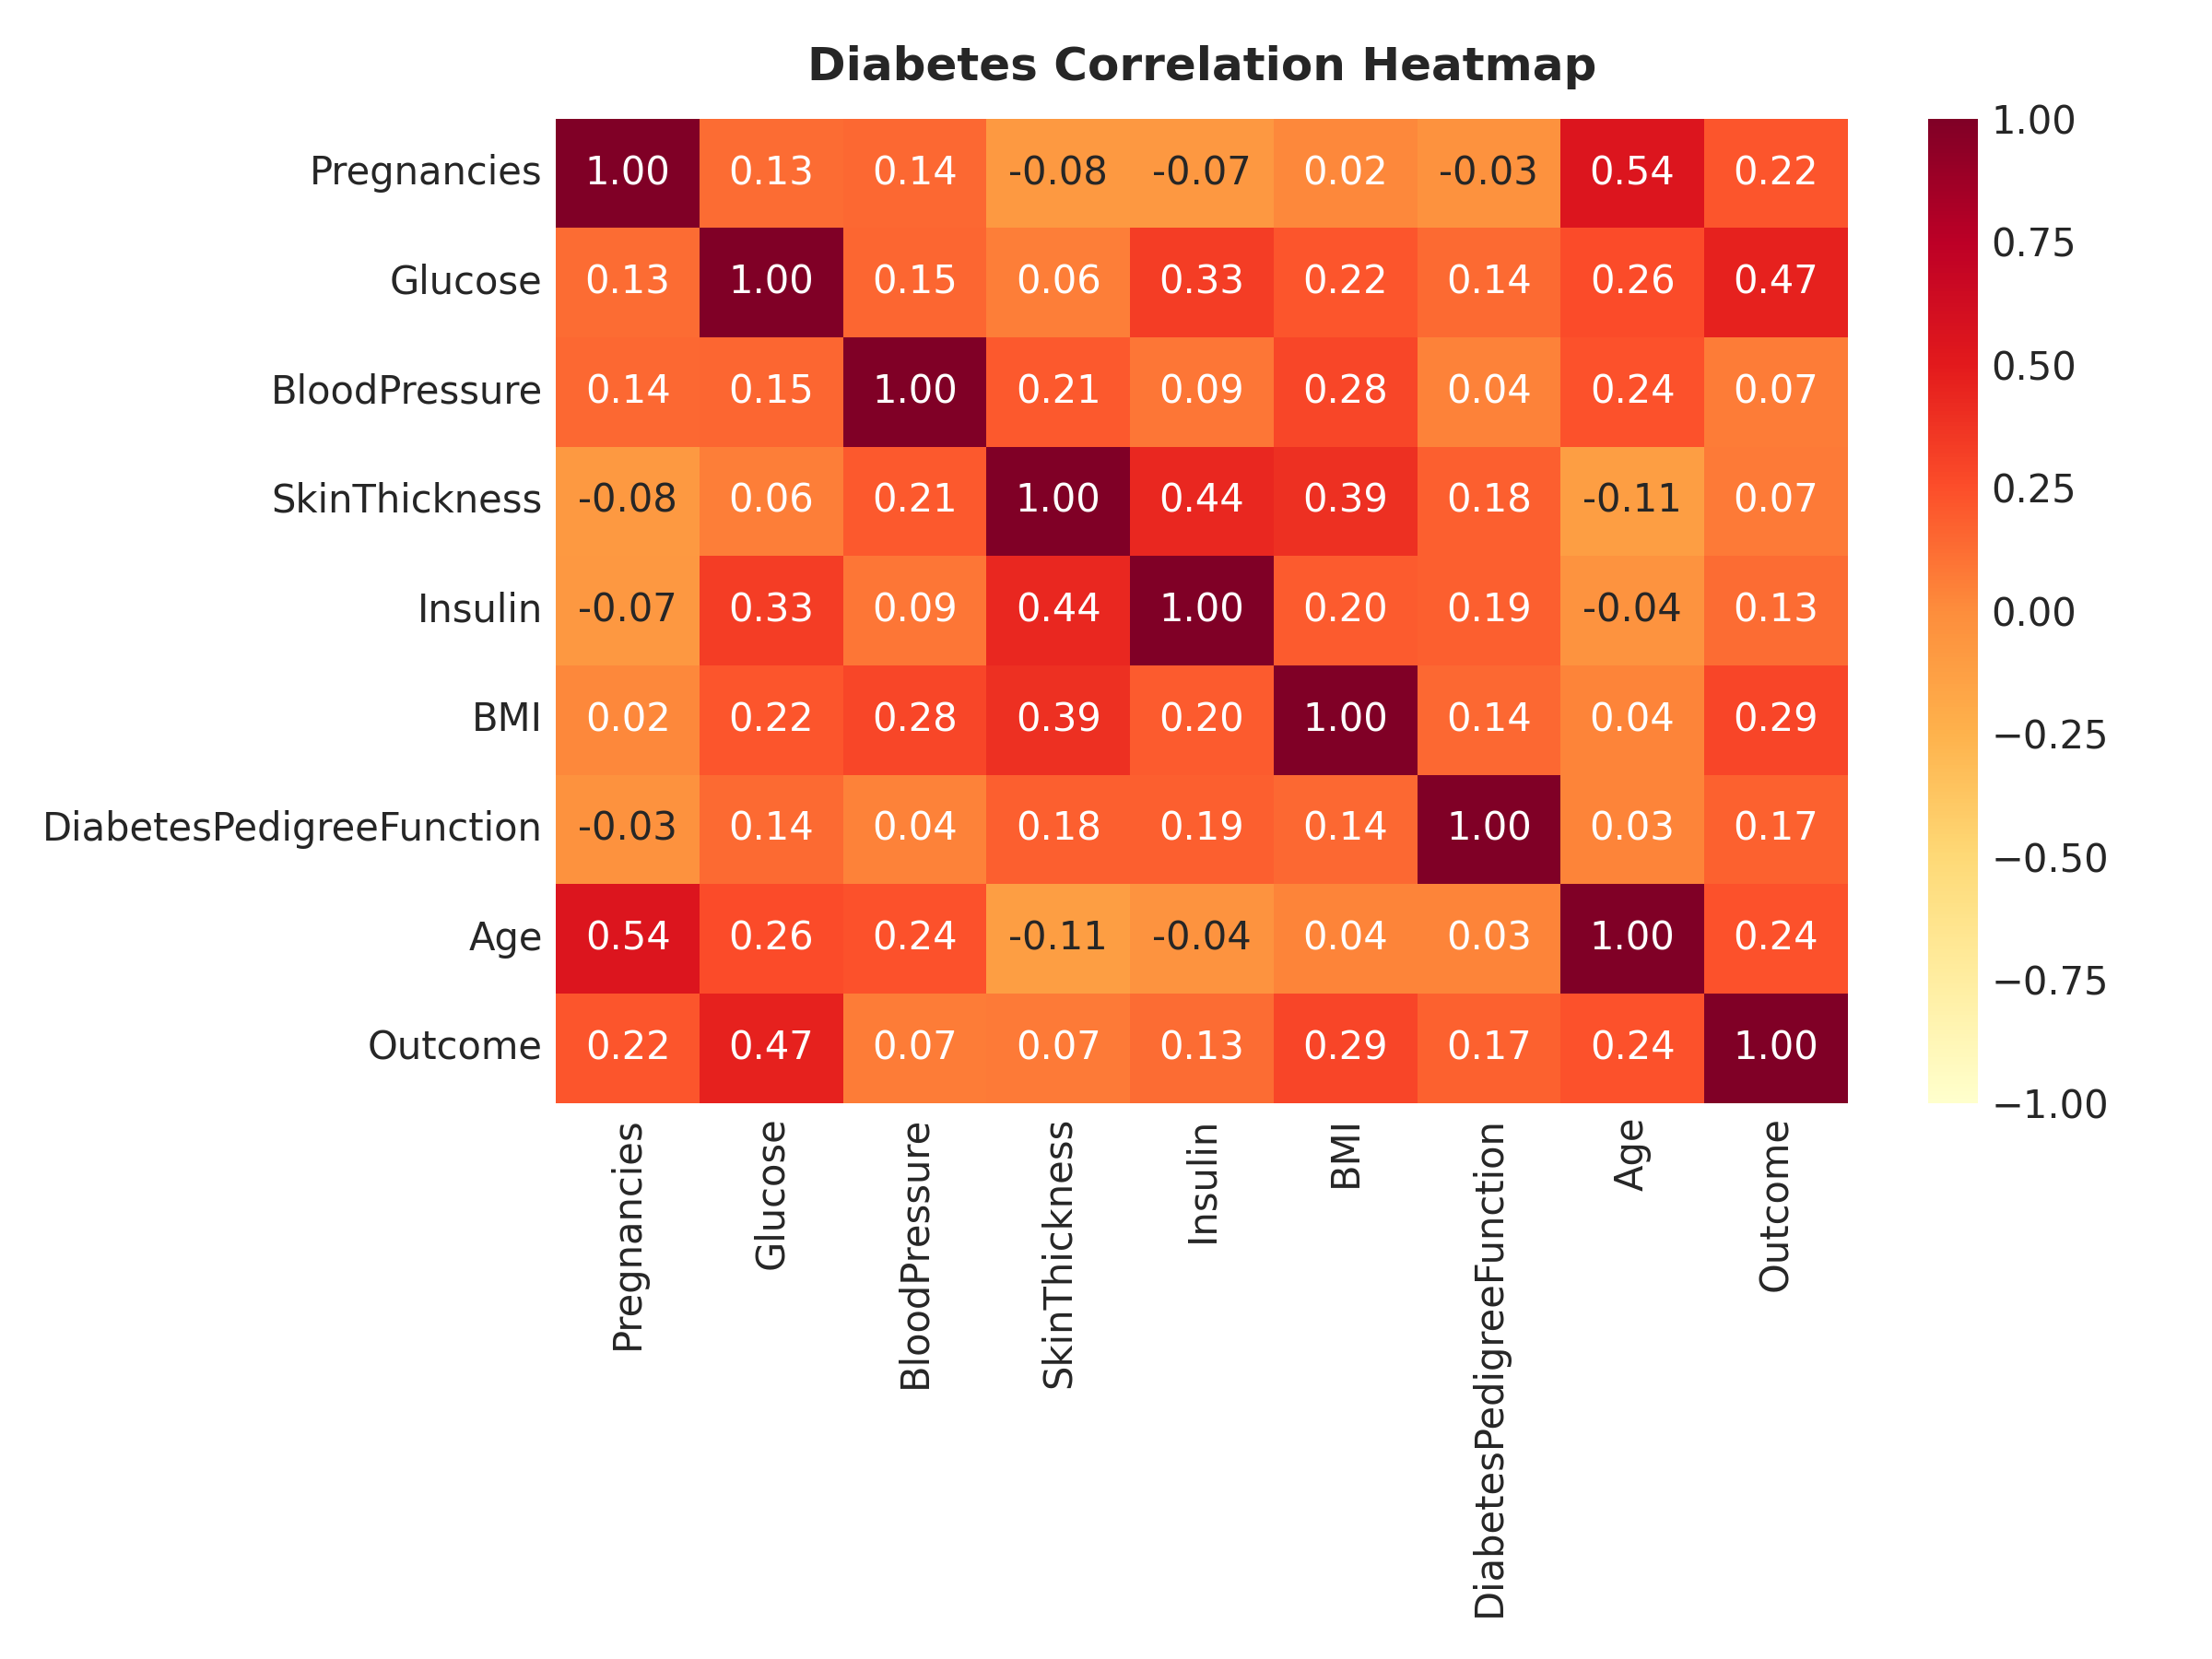
\includegraphics[width=0.75\linewidth]{figures_diabetes/correlation_heatmap.png}
\caption{Correlation Heatmap of Diabetes Attributes}
\label{fig:diab_correlation_heatmap}
\end{figure}
\textbf{Inference:} Glucose shows the highest positive linear correlation with Outcome ($r = 0.47$), followed by BMI ($r = 0.29$), Age ($r = 0.24$), and Pregnancies ($r = 0.22$).

\subsection{Pairwise Scatter Matrix (Pair Plot)}

\begin{figure}[H]
\centering
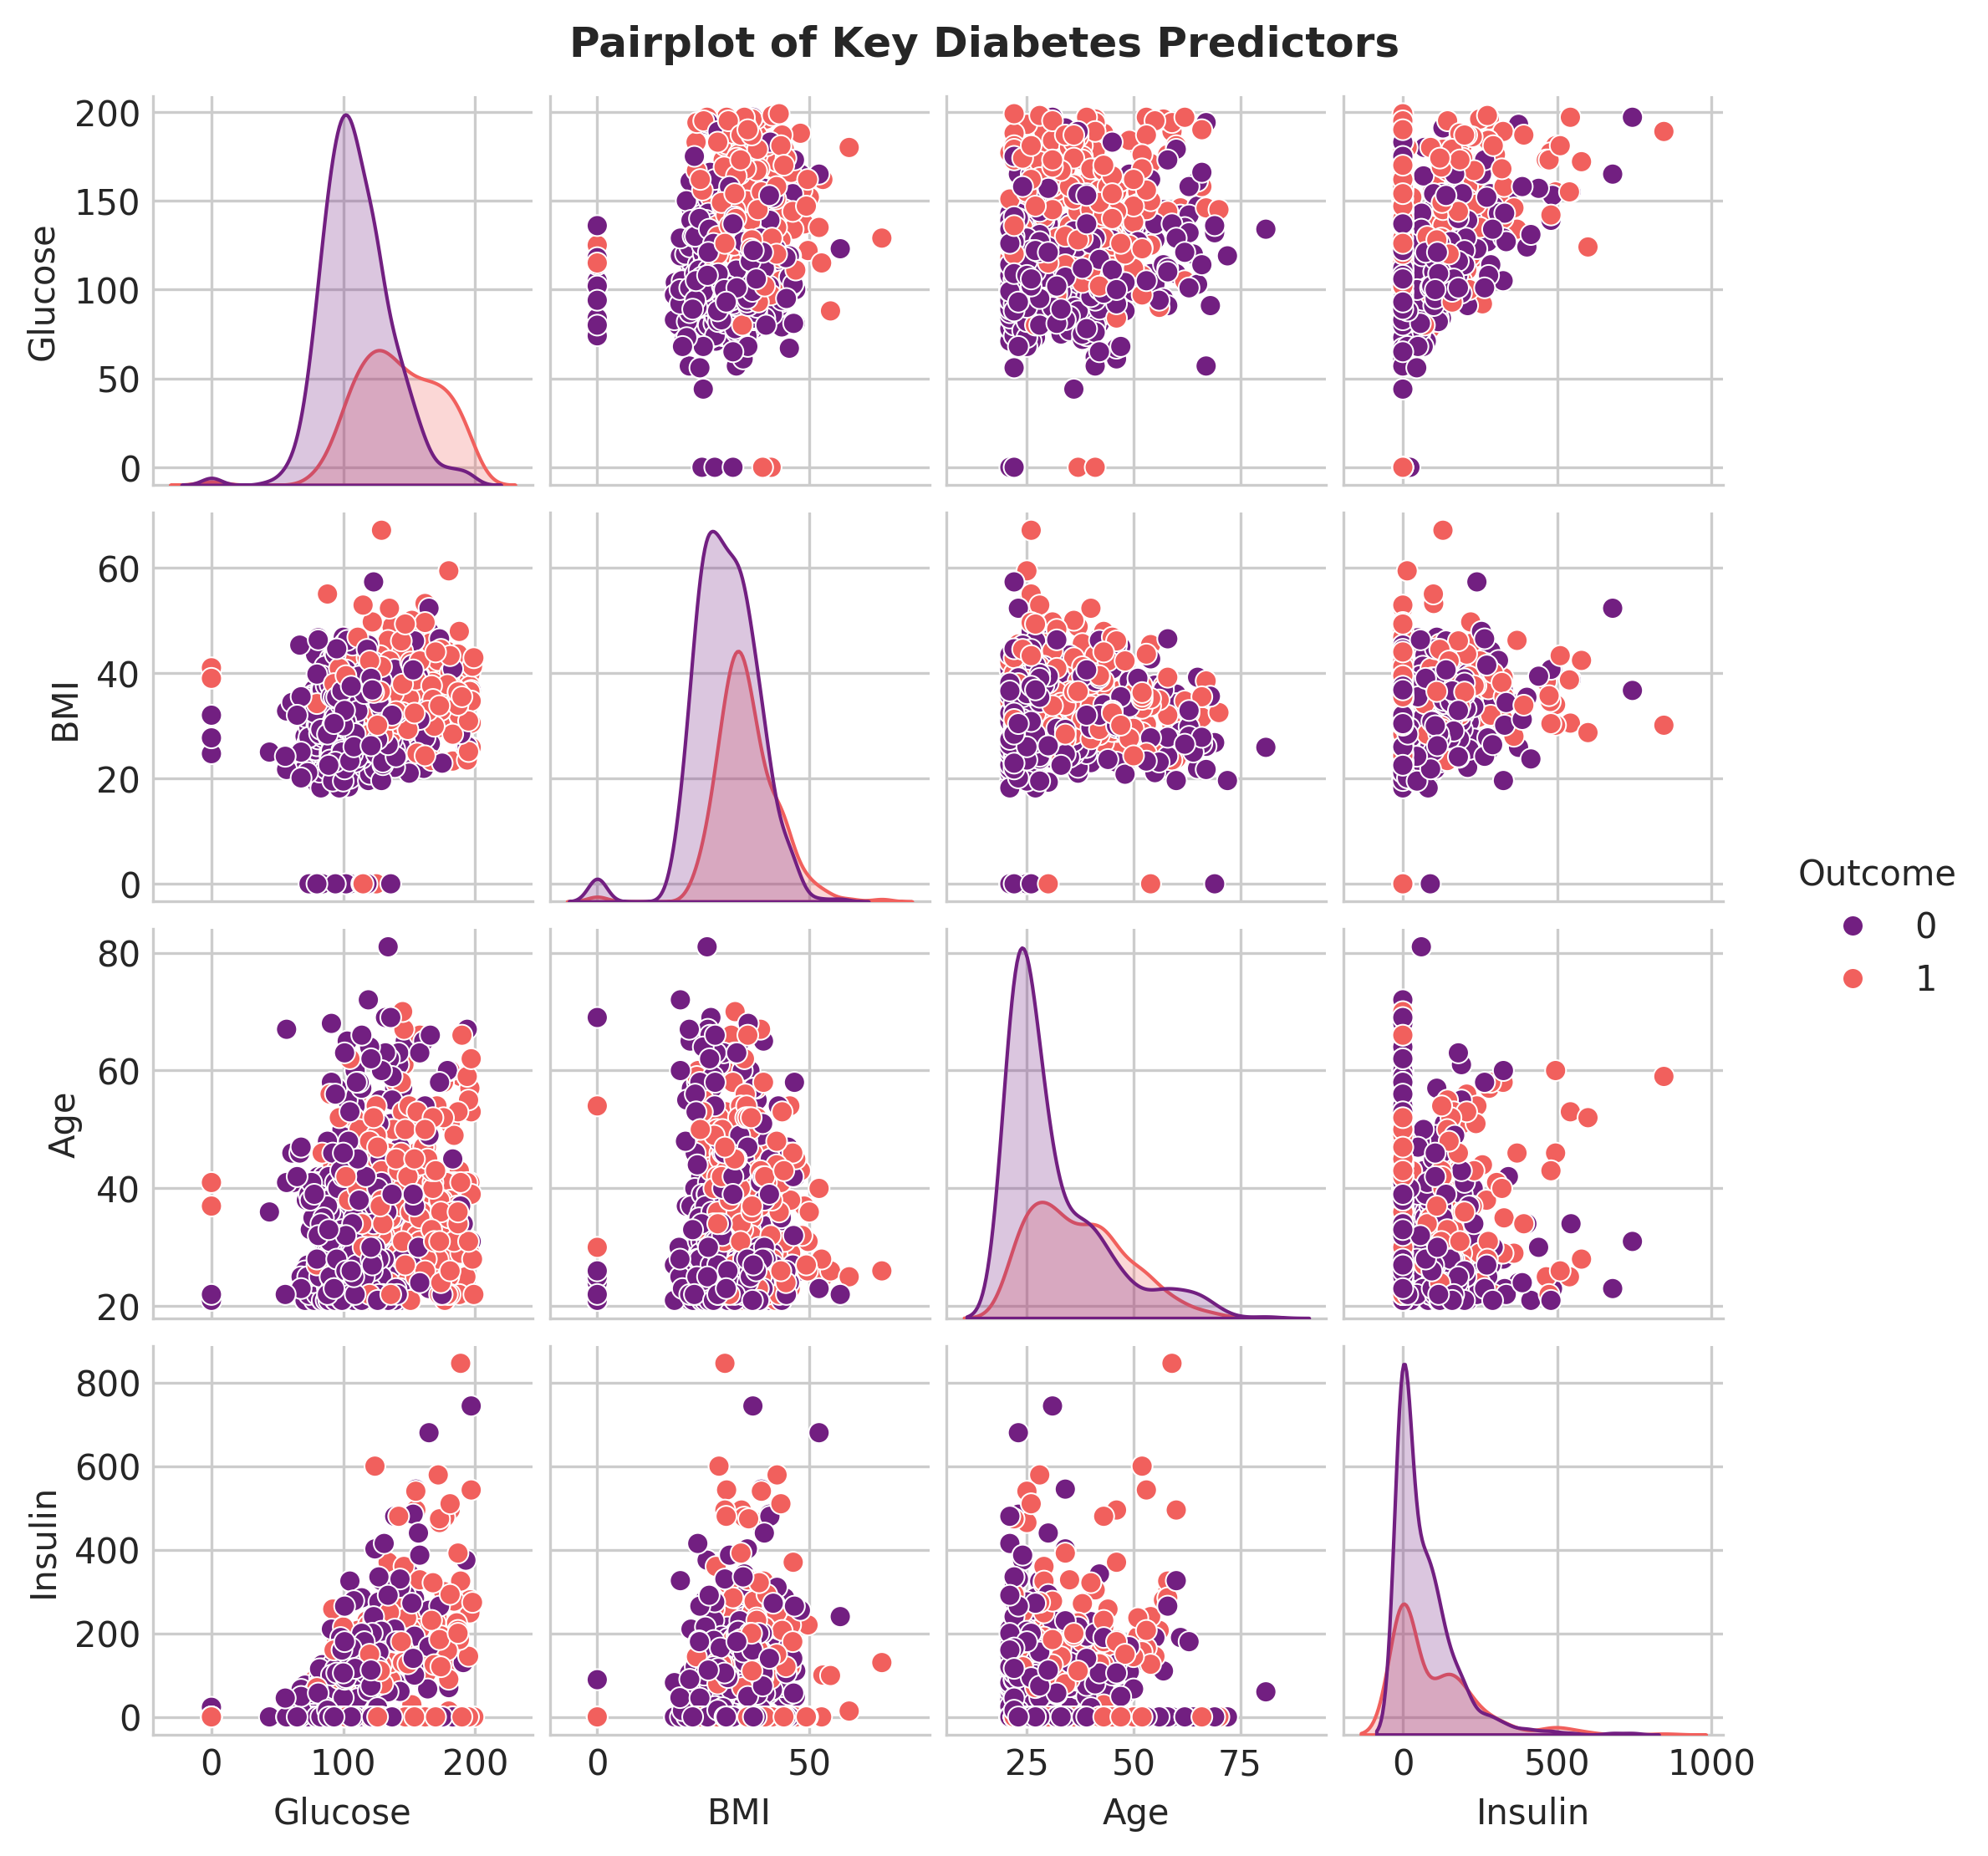
\includegraphics[width=0.75\linewidth]{figures_diabetes/pairplot.png}
\caption{Pair Plot of Key Diabetes Predictors}
\label{fig:diab_pairplot}
\end{figure}
\textbf{Inference:} Multi-attribute scatter projections demonstrate continuous dispersion between classes, emphasizing the need for non-linear decision boundaries.

\subsection{Bivariate Scatter Plots}

\begin{figure}[H]
\centering
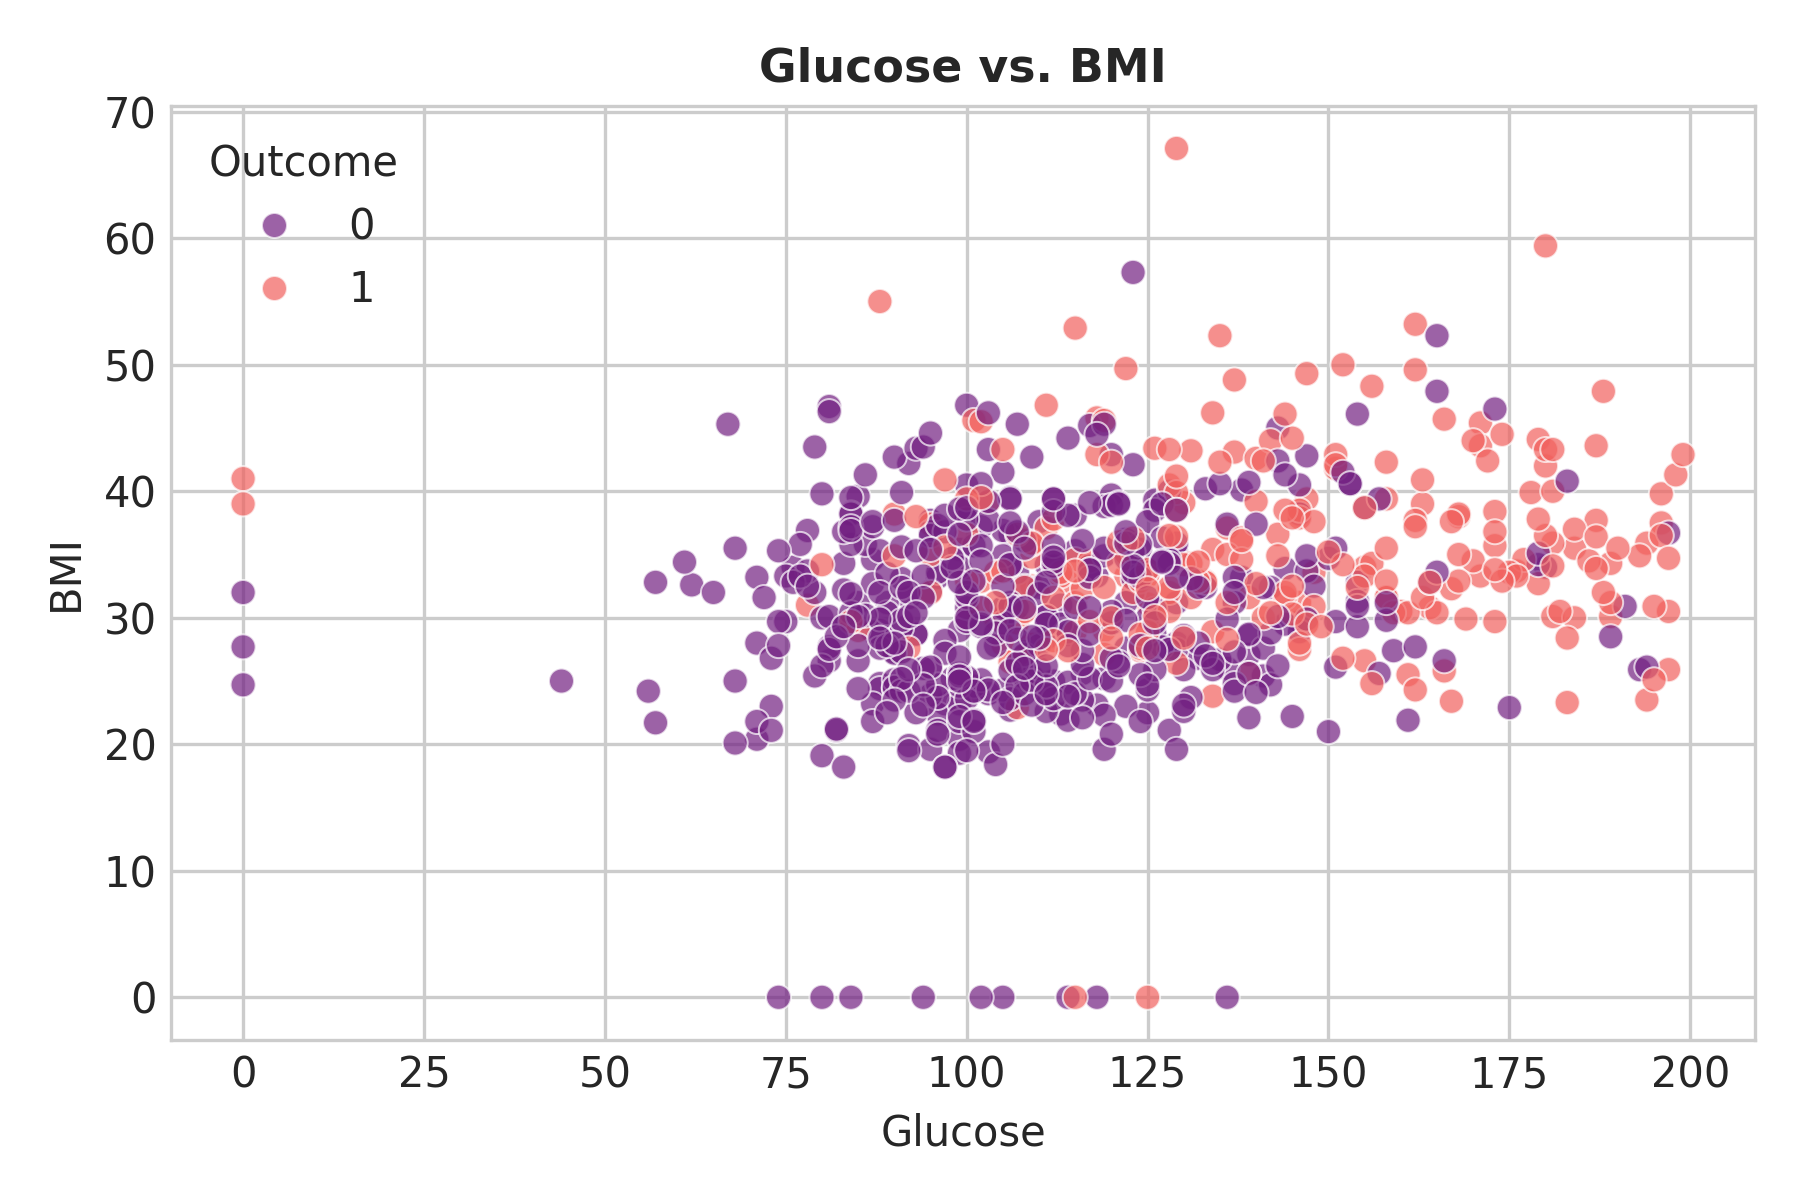
\includegraphics[width=0.75\linewidth]{figures_diabetes/scatter_Glucose_vs_BMI.png}
\caption{Scatter Plot: Glucose vs. BMI}
\label{fig:diab_scatter_glucose_bmi}
\end{figure}
\textbf{Inference:} Higher concentrations of diabetic outcomes appear in the upper-right quadrant (Glucose > 130 and BMI > 30).

\section{Data Preprocessing}
1. **Anomaly Handling**: Replace physiological zero values in Glucose, BloodPressure, SkinThickness, Insulin, and BMI with conditional median values.
2. **Feature Scaling**: Apply StandardScaler or RobustScaler to equalize feature variance prior to classifier training.

\section{Machine Learning Algorithms}
\begin{itemize}[noitemsep]
    \item \textbf{Suitable Algorithms}: Logistic Regression, Support Vector Classifier (SVC), Random Forest Classifier, XGBoost.
    \item \textbf{Feature Selection}: Chi-Square Test ($\chi^2$) or SelectKBest based on mutual information.
\end{itemize}

\section{Experimental Setup}
Executed via Python 3.10+ script environment with Seaborn and Matplotlib output engines.

\section{Hyperparameter Selection}
Plotting kernel bandwidths and boxplot whiskers were rendered using standard statistical parameters.

\section{Results}
All 29 diagnostic plots were generated cleanly and stored in \texttt{figures\_diabetes/}.

\section{Result Visualization}
Exploratory visualizations confirmed Glucose, BMI, and Age as the top three clinical discriminators for diabetes risk.

\section{Discussion}
Pre-processing physiological zero anomalies is vital for clinical diagnostic models to avoid biasing decision thresholds.

\section{Conclusion}
The automated EDA utility successfully highlighted key clinical indicators and missing value anomalies, establishing a pre-processed pipeline for diabetes risk prediction.

\section{References}
\begin{enumerate}[label={[\arabic*]}, leftmargin=2em]
    \item Smith, J. W., et al., ``Using the ADAP Learning Algorithm to Forecast the Onset of Diabetes Mellitus,'' *Proceedings of the Symposium on Computer Applications in Medical Care*, 1988.
    \item UCI Machine Learning Repository, ``Pima Indians Diabetes Database,'' \url{https://archive.ics.uci.edu/ml/datasets/pima+indians+diabetes}.
\end{enumerate}

\end{document}
